\chapter{Conditional Probability}
\label{chapter:ConditionalProbability}

Conditional probability provides a way to compute the likelihood of an event based on \emph{partial information}.
This is a powerful concept that is used extensively throughout engineering with applications to decision making, networks and digital communications.


\section{Conditioning on Events}

We begin our discussion of conditional probability with an illustrative example.
The intuition gained through this simple exercise is then generalized by introducing a formal definition for this important concept.

\begin{example}
The rolling of a fair die is an experiment with six equally likely outcomes.
As such, the probability of obtaining any of the outcomes is $1/6$.
However, if we are told that the upper face displays an odd number, then only three possibilities remain, namely $\{1, 3, 5 \}$.

\begin{center}

\includegraphics[height=3.675cm]{Figures/3Chapter/condevent}
\end{center}

These three outcomes had equal probabilities before the additional information was revealed.
It is natural to assume that they remain equally likely afterwards.
In particular, it is reasonable to assign a probability of $1/3$ to each of the three outcomes still plausible, in view of the new information.
Note that we can express the probability of getting, say, a three given that the outcome is an odd number as
\begin{equation*}
\begin{split}
\Pr (\text{3 given } \{ \text{odd numbers} \})
&= \frac{\Pr (\text{3 and } \{ \text{odd numbers} \})}
{\Pr (\text{odd numbers})} \\
&= \frac{\Pr(3)}{\Pr (\{1,3,5\})} = \frac{1}{3} .
\end{split}
\end{equation*}
\end{example}

Having reviewed a specific situation, we now turn to the more encompassing setting.
Let $B$ be an event such that $\Pr (B) > 0$.
A conditional probability law assigns to every event $A$ a number $\Pr (A|B)$, termed the \emph{conditional probability of $A$ given $B$}, such that \index{Conditional Probability}
\begin{equation} \label{equation:ConditionalProbability}
\Pr (A | B) = \frac{\Pr (A \cap B)}{\Pr (B)}.
\end{equation}
We can show that the set of conditional probabilities $\{ \Pr (A | B) \}$ specifies a valid probability law, as defined in Section~\ref{section:ProbabilityLaws}.
For every event $A$, we have
\begin{equation*}
\Pr (A|B) = \frac{\Pr (A \cap B)}{\Pr (B)} \geq 0.
\end{equation*}
That is, $\Pr (A|B)$ is nonnegative.
The probability of the entire sample space $\Omega$ is equal to
\begin{equation*}
\Pr (\Omega | B) = \frac{\Pr (\Omega \cap B)}{\Pr (B)}
= \frac{\Pr (B)}{\Pr (B)} = 1 .
\end{equation*}
If $A_1, A_2, \ldots$ is a sequence of disjoint events, then
\begin{equation*}
A_1 \cap B, A_2 \cap B, \ldots
\end{equation*}
is also a sequence of disjoint events and
\begin{equation*}
\begin{split}
\Pr \left( \bigcup_{k=1}^{\infty} A_k \Big| B \right)
&= \frac{\Pr \left( \left( \bigcup_{k=1}^{\infty} A_k \right) \cap B \right)}{\Pr (B)}
= \frac{\Pr \left( \bigcup_{k=1}^{\infty} (A_k \cap B ) \right)}{\Pr (B)} \\
&= \sum_{k = 1}^{\infty} \frac{ \Pr (A_k \cap B ) }{\Pr (B)}
= \sum_{k = 1}^{\infty} \Pr (A_k | B) ,
\end{split}
\end{equation*}
where the third equality follows from the third axiom of probability applied to the set $\bigcup_{k=1}^{\infty} (A_k \cap B )$.
Hence, the conditional probability law defined by \eqref{equation:ConditionalProbability} satisfies the three axioms of probability.

\begin{example}
A fair coin is tossed repetitively until heads is observed.
In Example~\ref{example:CoinTossSequence}, we found that the probability of observing heads for the first time on trial $n$ is $2^{-k}$.
We now wish to compute the probability that heads occurred for the first time on the second trial given that it took an even number of tosses to observe heads.
In this example, $A = \{ 2 \}$ and $B$ is the set of even numbers.
The probability that the outcome is two given that the number of tosses is even is equal to
\begin{equation*}
\begin{split}
\Pr ( 2 | \text{even numbers} )
&= \frac{\Pr ( 2 \cap \{ \text{even numbers} \} )}
{\Pr (\text{even numbers})} \\
&= \frac{\Pr (2)}{\Pr (\text{even numbers})} \\
&= \frac{1/4}{1/3}
= \frac{3}{4} .
\end{split}
\end{equation*}
In the above computation, we have used the fact that the probability of flipping the coin an even number of times is equal to $1/3$.
This fact was obtained in Example~\ref{example:CoinTossSequence}.
\end{example}

The definition of conditional probability can be employed to compute the probability of several events occurring simultaneously.
Let $A_1, A_2, \ldots, A_n$ be a collection of events.
The probability of events $A_1$ through $A_n$ taking place at the same time is given by
\begin{equation} \label{equation:SimultaneousEvents}
\Pr \left( \bigcap_{k=1}^n A_k \right)
= \Pr (A_1) \Pr (A_2 | A_1) \Pr (A_3 | A_1 \cap A_2)
\cdots \Pr \left( A_n \bigg| \bigcap_{k=1}^{n-1} A_k \right) .
\end{equation}
This formula can be verified by expanding each of the conditional probabilities using \eqref{equation:ConditionalProbability},
\begin{equation*}
\Pr \left( \bigcap_{k=1}^n A_k \right)
= \Pr (A_1) \frac{\Pr (A_2 \cap A_1)}{\Pr (A_1)}
\frac{\Pr (A_1 \cap A_2 \cap A_3)}{\Pr (A_1 \cap A_2)}
\cdots \frac{\Pr \left( \bigcap_{k=1}^{n} A_k \right)}
{\Pr \left( \bigcap_{k=1}^{n-1} A_k \right)} .
\end{equation*}

\begin{example}
An urn contains eight blue balls and four green balls.
Three balls are drawn from this urn without replacement.
We wish to compute the probability that all three balls are blue.
The probability of drawing a blue ball the first time is equal to $8/12$.
The probability of drawing a blue ball the second time given that the first ball is blue is $7/11$.
Finally, the probability of drawing a blue ball the third time given that the previous two balls are blue is $6/10$.
Using \eqref{equation:SimultaneousEvents}, we can compute the probability drawing three blue balls as
\begin{equation*}
\Pr (\text{3 blue balls})
= \frac{8}{12} \frac{7}{11} \frac{6}{10}
= \frac{14}{55} .
\end{equation*}

\begin{center}
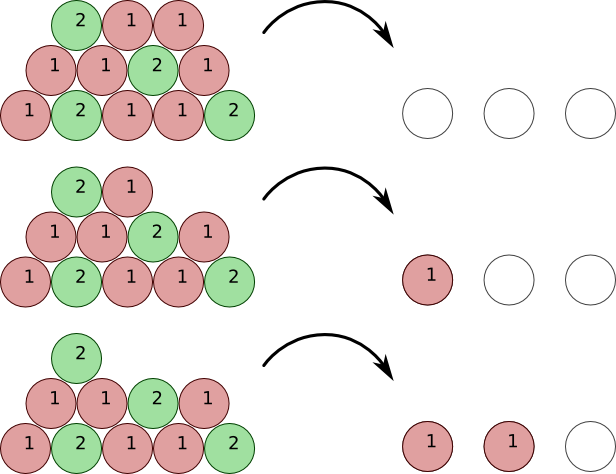
\includegraphics[height=7.11cm]{Figures/3Chapter/balls}
\end{center}
\end{example}


\section{The Total Probability Theorem}

The probability of events $A$ and $B$ occurring at the same time can be calculated as a special case of \eqref{equation:SimultaneousEvents}.
For two events, this computational formula simplifies to
\begin{equation} \label{equation:ProbabilityIntersection}
\Pr (A \cap B) = \Pr (A|B) \Pr (B) .
\end{equation}
We can also obtain this equation directly from the definition of conditional probability.
This property is a key observation that plays a central role in establishing two important results, the \emph{total probability theorem} and \emph{Bayes' rule}.
To formulate these two theorems, we need to revisit the notion of a partition.
A collection of events $A_1, A_2, \ldots, A_n$ is said to be a \emph{partition} of the sample space $\Omega$ if these events are disjoint and their union is the entire sample space, \index{Partition}
\begin{equation*}
\bigcup_{k=1}^n A_k = \Omega .
\end{equation*}
Visually, a partition divides an entire set into disjoint subsets.
\begin{center}
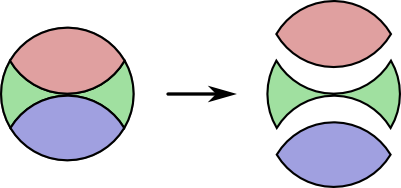
\includegraphics[height=4.23cm]{Figures/3Chapter/setpartition2}
\end{center}

\begin{theorem}[Total Probability Theorem] \label{theorem:TotalProbability} \index{Total Probability Theorem}
Let $A_1, A_2, \ldots, A_n$ be a collection of events that forms a partition of the sample space $\Omega$.
Suppose that $\Pr (A_k) > 0$ for all $k$.
Then, for any event $B$, we can write
\begin{equation*}
\begin{split}
\Pr (B) &= \Pr (A_1 \cap B) + \Pr (A_2 \cap B) + \cdots + \Pr (A_n \cap B) \\
&= \Pr (A_1) \Pr (B | A_1) + \Pr (A_2) \Pr (B | A_2) + \cdots + \Pr (A_n) \Pr (B | A_n ) .
\end{split}
\end{equation*}
\end{theorem}
\begin{proof}
The collection of events $A_1, A_2, \ldots, A_n$ forms a partition of the sample space $\Omega$.
We can therefore write
\begin{equation*}
B = B \cap \Omega = B \cap \left( \bigcup_{k=1}^n A_k \right) .
\end{equation*}
Since $A_1, A_2, \ldots, A_n$ are disjoint sets, the events
\begin{equation*}
A_1 \cap B, A_2 \cap B, \ldots, A_n \cap B
\end{equation*}
are also disjoint.
Combining these two facts, we get
\begin{equation*}
\begin{split}
\Pr (B)
&= \Pr \left( B \cap \left( \bigcup_{k=1}^n A_k \right) \right)
= \Pr \left( \bigcup_{k=1}^n (B \cap A_k) \right) \\
&= \sum_{k=1}^n \Pr \left( B \cap A_k \right)
= \sum_{k=1}^n \Pr (A_k) \Pr \left( B |A_k \right) ,
\end{split}
\end{equation*}
where the fourth equality is obtained by applying the third axiom of probability.
\end{proof}

\begin{center}
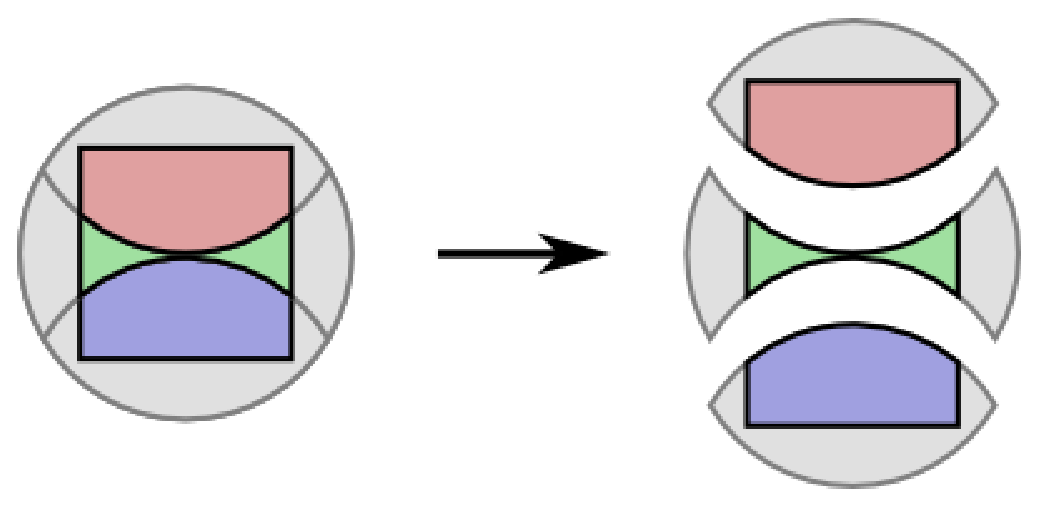
\includegraphics[height=4.23cm]{Figures/3Chapter/setpartition3}
\end{center}
A graphical interpretation of Theorem~\ref{theorem:TotalProbability} is illustrated above.
Event $B$ can be decomposed into the disjoint union of $A_1 \cap B, A_2 \cap B, \ldots, A_n \cap B$.
The probability of event $B$ can then be computed by adding these various parts
\begin{equation*}
\Pr (A_1 \cap B), \Pr (A_2 \cap B), \ldots, \Pr (A_n \cap B) .
\end{equation*}

\begin{example}
An urn contains eight blue balls and four red balls.
A first ball is drawn from the urn.
If this ball is red then the experiment stops, otherwise one more ball is drawn from the urn.
What is the probability of obtaining a red ball?

In this problem, there are three outcomes of interest.
If we denote the drawing of a red ball by $r$ and the drawing of a blue ball by $b$, then these three outcomes can be represented by $\{ r, br, bb \}$.
The probability of drawing a red ball initially is $\Pr (r) = 4/12$.
The probabilities of drawing two balls can be computed using \eqref{equation:SimultaneousEvents}, and they are given by
\begin{align*}
\Pr (br) &= \frac{8}{12} \frac{4}{11} = \frac{8}{33} \\
\Pr (bb) &= \frac{8}{12} \frac{7}{11} = \frac{14}{33} .
\end{align*}
Let $R$ denote the event that a red ball is obtained during the experiment.
The overall probability of getting a red ball, $\Pr (R)$, can be computed by applying the total probability theorem
\begin{equation*}
\begin{split}
\Pr (R) &= \Pr (R \cap r) + \Pr (R \cap br) + \Pr (R \cap bb) \\
&= \Pr(r) \Pr (R|r) + \Pr(br) \Pr (R|br) + \Pr(bb) \Pr (R|bb) \\
&= \frac{1}{3} \cdot 1 + \frac{8}{33} \cdot 1 + \frac{14}{33} \cdot 0
= \frac{19}{33} .
\end{split}
\end{equation*}
\end{example}


\section{Bayes' Rule}

The following result is also very useful.
It relates the conditional probability of $A$ given $B$ to the conditional probability of $B$ given $A$.

\begin{theorem}[Bayes' Rule] \index{Bayes' Rule}
Let $A_1, A_2, \ldots, A_n$ be a collection of events that forms a partition of the sample space $\Omega$.
Suppose that $\Pr (A_k) > 0$ for all $k$.
Then, for any event $B$ such that $\Pr (B) > 0$, we can write
\begin{equation*}
\begin{split}
\Pr (A_i | B)
&= \frac{ \Pr (A_i) \Pr (B | A_i) }{ \Pr (B) } \\
&= \frac{ \Pr (A_i) \Pr (B | A_i) }
{ \sum_{k=1}^n \Pr (A_k) \Pr (B | A_k) } .
\end{split}
\end{equation*}
\end{theorem}
\begin{proof}
Bayes' rule is easily verified.
We expand the probability of $A_i \cap B$ using \eqref{equation:ProbabilityIntersection} twice, and we get
\begin{equation*}
\Pr (A_i \cap B) = \Pr (A_i | B) \Pr (B) = \Pr (B | A_i) \Pr (A_i).
\end{equation*}
Rearranging the terms yields the first equality.
The second equality is obtained by writing
\begin{equation*}
\begin{split}
\Pr (B) &= \Pr (B \cap \Omega)
= \Pr \left( B \cap \left( \bigcup_{k=1}^n A_k \right) \right) \\
&= \sum_{k=1}^n \Pr (B \cap A_k)
= \sum_{k=1}^n \Pr (A_k) \Pr (B | A_k) .
\end{split}
\end{equation*}
The application of the third axiom of probability is justified because
\begin{equation*}
A_1, A_2, \ldots, A_n
\end{equation*}
are disjoint events.
\end{proof}

\begin{example}
April, a biochemist, designs a test for a latent disease.
If a subject has the disease, the probability that the test results are positive is $0.95$.
Similarly, if a subject does not have the disease, the probability that the test results are negative is $0.95$.
Suppose that one percent of the population has the disease.
We wish to find the probability that a person who tested positive has the disease.

Let $D$ denote the event that the person has the disease, and let $P$ be the event that the test results are positive.
Using Bayes' rule, we can easily compute the probability that a person who tested positive has the disease,
\begin{equation*}
\begin{split}
\Pr (D|P)
&= \frac{ \Pr(D) \Pr(P|D) }{ \Pr(D) \Pr(P|D) + \Pr(D^{\Complement}) \Pr(P|D^{\Complement}) } \\
&= \frac{ 0.01 \cdot 0.95 }{ 0.01 \cdot 0.95 + 0.99 \cdot 0.05 } \\
&\approx 0.1610 .
\end{split}
\end{equation*}
Although the test is fairly accurate, the probability that a person with a positive test carries the disease remains small.
\end{example}


\section{Independence}
\label{section:Independence}

Events $A$ and $B$ are said to be \emph{independent} if $\Pr (A \cap B) = \Pr(A) \Pr(B)$. \index{Independence}
Interestingly, independence is closely linked to the concept of conditional probability.
If $\Pr(B) > 0$ and events $A$ and $B$ are independent, then
\begin{equation*}
\Pr (A | B) = \frac{ \Pr (A \cap B) }{\Pr (B)}
= \frac{ \Pr (A) \Pr(B) }{\Pr (B)}
= \Pr (A).
\end{equation*}
The \emph{a priori} probability of event $A$ is identical to the \emph{a posteriori} probability of $A$ given $B$.
That is, if $A$ is independent of $B$, then partial knowledge about $B$ contains no information on the likely occurrence of $A$.
We note that independence is a symmetric relation; if $A$ is independent of $B$, then $B$ is also independent of $A$.
It is therefore unambiguous to say that $A$ and $B$ are independent events.

\begin{example}
Suppose that two dice are rolled at the same time, a red die and a blue die.
We observe the numbers that appear on the upper faces of the two dice.
The sample space for this experiment is composed of thirty-six equally likely outcomes.
Consider the probability of getting a four on the red die given that the blue die shows a six,
\begin{equation*}
\begin{split}
\Pr (\text{red = 4} | \text{blue = 6})
&= \frac{ \Pr (\text{red = 4} \cap \text{blue = 6}) }
{ \Pr (\text{blue = 6}) } \\
&= \frac{1}{6} = \Pr (\text{red = 4}) .
\end{split}
\end{equation*}
From this equation, we gather that
\begin{equation*}
\Pr (\text{red = 4} \cap \text{blue = 6})
= \Pr (\text{red = 4}) \Pr (\text{blue = 6}) .
\end{equation*}
Thus, rolling a four on the red die and rolling a six on the blue die are independent events.

Similarly, consider the probability of obtaining a four on the red die given that the sum of the two dice is eleven,
\begin{equation*}
\begin{split}
\Pr (\text{red = 4} | \text{sum = 11})
&= \frac{ \Pr (\text{red = 4} \cap \text{sum = 11}) }
{ \Pr (\text{sum = 11}) } = 0 \\
&\neq \frac{1}{6} = \Pr (\text{red = 4}) .
\end{split}
\end{equation*}
In this case, we conclude that getting a four on the red die and a sum total of eleven are not independent events.
\end{example}

The basic idea of independence seems intuitively clear: if knowledge about the occurrence of event $B$ has no impact on the probability of $A$, then these two events must be independent.
Yet independent events are not necessarily easy to visualize in terms of the sample space.
A common mistake is to assume that two events are independent if they are disjoint.
Two mutually exclusive events can hardly be independent.
If $\Pr (A) > 0$, $\Pr (B) > 0$, and $\Pr (A \cap B) = 0$ then
\begin{equation*}
\Pr (A \cap B) = 0 < \Pr (A) \Pr(B).
\end{equation*}
Thus, $A$ and $B$ cannot be independent if they are disjoint, non-trivial sets.


\subsection{Independence of Multiple Events}

The concept of independence can be extended to multiple events.
The events $A_1, A_2, \ldots, A_n$ are \emph{independent} provided that \index{Independence}
\begin{equation} \label{equation:IndependenceMultipleEvents}
\Pr \left( \bigcap_{i \in \IndexSet} A_i \right)
= \prod_{i \in \IndexSet} \Pr (A_i) ,
\end{equation}
for every subset $\IndexSet$ of $\{1, 2, \ldots, n\}$.

For instance, consider a collection of three events, $A$, $B$ and $C$.
These events are independent if
\begin{equation} \label{equation:ThreeIndependentEvents}
\begin{split}
\Pr (A \cap B) &= \Pr (A) \Pr (B) \\
\Pr (A \cap C) &= \Pr (A) \Pr (C) \\
\Pr (B \cap C) &= \Pr (B) \Pr (C)
\end{split}
\end{equation}
and, in addition,
\begin{equation*}
\Pr (A \cap B \cap C) = \Pr (A) \Pr (B) \Pr(C) .
\end{equation*}
The three equalities in \eqref{equation:ThreeIndependentEvents} assert that $A$, $B$ and $C$ are \emph{pairwise independent}.
Note that the fourth condition does not follow from the first three conditions, nor does it imply any of them.
Pairwise independence does not imply independence.

\begin{example}
A fair coin is flipped twice.
Let $A$ denote the event that heads is observed on the first toss.
Let $B$ be the event that heads is obtained on the second toss.
Finally, let $C$ be the event that the two coins show distinct sides.
These three events each have a probability of $1/2$.
Furthermore, we have
\begin{equation*}
\Pr (A \cap B) = \Pr (A \cap C) = \Pr (B \cap C) = \frac{1}{4} .
\end{equation*}
That is, these events are pairwise independent.
However, we can verify that
\begin{equation*}
\Pr (A \cap B \cap C) = 0 \neq \frac{1}{8} = \Pr (A) \Pr (B) \Pr (C) .
\end{equation*}
This shows that events $A$, $B$ and $C$ are not independent.
\end{example}

\begin{example}
Two dice are rolled at the same time, a red die and a blue die.
Let $A$ be the event that the number on the red die is odd.
Let $B$ be the event that the number on the red die is either two, three or four.
Also, let $C$ be the event that the product of the two dice is twelve.
The individual probabilities of these events are
\begin{align*}
\Pr (A) &= \Pr (\text{red is odd}) = \frac{1}{2} \\
\Pr (B) &= \Pr (\text{red} \in \{2, 3, 4\}) = \frac{1}{2} \\
\Pr (C) &= \Pr (\text{product = 12}) = \frac{4}{36} .
\end{align*}
We note that these events are not pairwise independent because
\begin{align*}
\Pr (A \cap B) &= \frac{1}{6} \neq \frac{1}{4} = \Pr(A) \Pr(B) \\
\Pr (A \cap C) &= \frac{1}{36} \neq \frac{1}{18} = \Pr(A) \Pr(C) \\
\Pr (B \cap C) &= \frac{1}{12} \neq \frac{1}{18} = \Pr(B) \Pr(C) .
\end{align*}
The multiple events $A$, $B$ and $C$ are not independent.
On the other hand, the probability of these three events occurring simultaneously is
\begin{equation*}
\Pr (A \cap B \cap C) = \frac{1}{36}
= \frac{1}{2} \cdot \frac{1}{2} \cdot \frac{4}{36}
= \Pr (A) \Pr (B) \Pr (C) .
\end{equation*}
\end{example}

\subsection{Conditional Independence}

We introduced earlier the meaning of conditional probability, and we showed that the set of conditional probabilities $\{ \Pr (A|B) \}$ specifies a valid probability law.
It is therefore possible to discuss independence with respect to conditional probability.
We say that events $A_1$ and $A_2$ are \emph{conditionally independent} if \index{Conditional Independence}
\begin{equation*}
\Pr (A_1 \cap A_2 | B) = \Pr (A_1 | B) \Pr (A_2 | B) .
\end{equation*}
Note that if $A_1$ and $A_2$ are conditionally independent given event $B$, we can use equation \eqref{equation:ConditionalProbability} to write
\begin{equation*}
\begin{split}
\Pr (A_1 \cap A_2 | B) &= \frac{ \Pr (A_1 \cap A_2 \cap  B) }{\Pr (B)} \\
&= \frac{ \Pr (B) \Pr (A_1 | B) \Pr (A_2 | A_1 \cap  B) }{\Pr (B)} \\
&= \Pr (A_1 | B) \Pr (A_2 | A_1 \cap  B) .
\end{split}
\end{equation*}
Under the assumption that $\Pr (A_1 | B) > 0$, we can combine the previous two expressions and get
\begin{equation*}
\Pr (A_2 | A_1 \cap  B) = \Pr (A_2 | B) .
\end{equation*}
This latter result asserts that, given event $B$ has taken place, the additional information that $A_1$ also occurred does not affect the conditional probability of $A_2$.
It is simple to show that conditional independence is a symmetric relation as well.

\begin{example}
Suppose that a fair coin is tossed until heads is observed.
The number of trials is recorded as the outcome of this experiment.
We denote by $B$ the event that the coin is tossed more than one time.
Moreover, we let $A_1$ be the event that the number of trials is an even number, and $A_2$ be the event that the number of trials is less than six.
The conditional probabilities of $A_1$ and $A_2$ given that the coin is tossed more than once are
\begin{align*}
\Pr (A_1 | B) &= \frac{ \Pr (A_1 \cap B) }{ \Pr (B) }
= \frac{1/3}{1/2} = \frac{2}{3} \\
\Pr (A_2 | B) &= \frac{ \Pr (A_2 \cap B) }{ \Pr (B) }
= \frac{15/32}{1/2} = \frac{15}{16} .
\end{align*}
The joint probability of events $A_1$ and $A_2$ given $B$ is equal to
\begin{equation*}
\begin{split}
\Pr (A_1 \cap A_2 | B) &= \frac{ \Pr (A_1 \cap A_2 \cap B) }{ \Pr (B) } \\
&= \frac{5/16}{1/2} = \frac{5}{8} = \frac{2}{3} \cdot \frac{15}{16} \\
&= \Pr (A_1 | B) \Pr (A_2 | B) .
\end{split}
\end{equation*}
It follows that $A_1$ and $A_2$ are conditionally independent given $B$.
In particular, we have
\begin{align*}
\Pr (A_2 | A_1 \cap  B) &= \Pr (A_2 | B) \\
\Pr (A_1 | A_2 \cap  B) &= \Pr (A_1 | B) .
\end{align*}
We emphasize that events $A_1$ and $A_2$ are not independent with respect to the unconditional probability law.
\end{example}

Two events that are independent with respect to an unconditional probability law, may not be conditionally independent.

\begin{example}
Two dice are rolled at the same time, a red die and a blue die.
We can easily compute the probability of simultaneously getting a two on the red die and a six on the blue die,
\begin{equation*}
\Pr (\text{red = 2} \cap \text{blue = 6}) = \frac{1}{36}
= \Pr (\text{red = 2}) \Pr (\text{blue = 6}) .
\end{equation*}
Clearly, these two events are independent.

Now, consider the probability of rolling a two on the red die and a six on the blue die given that the sum of the two dice is an odd number.
The individual conditional probabilities are given by
\begin{equation*}
\Pr (\text{red = 2} | \text{sum is odd})
= \Pr (\text{blue = 6} | \text{sum is odd})
= \frac{1}{6},
\end{equation*}
whereas the joint conditional probability is
\begin{equation*}
\Pr (\text{red = 2} \cap \text{blue = 6} | \text{sum is odd})
= 0 .
\end{equation*}
These two events are not conditionally independent.
\end{example}

It is possible to extend the notion of conditional independence to several events.
The events $A_1, A_2, \ldots, A_n$ are conditionally independent given $B$ if
\begin{equation*}
\Pr \left( \bigcap_{i \in \IndexSet} A_i \Big| B \right)
= \prod_{i \in \IndexSet} \Pr (A_i | B)
\end{equation*}
for every subset $\IndexSet$ of $\{1, 2, \ldots, n\}$.
This definition is analogous to \eqref{equation:IndependenceMultipleEvents}, albeit using the proper conditional probability law.


\section{Equivalent Notations}

In the study of probability, we are frequently interested in the probability of multiple events occurring simultaneously.
So far, we have expressed the joint probability of events $A$ and $B$ using the notation $\Pr (A \cap B)$.
For mathematical convenience, we also represent the probability that two events occur at the same time by
\begin{equation*}
\Pr (A, B) = \Pr (A \cap B) .
\end{equation*}
This alternate notation easily extends to the joint probability of several events.
We denote the joint probability of events $A_1, A_2, \ldots, A_n$ by
\begin{equation*}
\Pr (A_1, A_2, \ldots, A_n) =
\Pr \left( \bigcap_{k=1}^n A_k \right) .
\end{equation*}
Conditional probabilities can be written using a similar format.
The probability of $A$ given events $B_1, B_2, \ldots, B_n$ becomes
\begin{equation*}
\Pr (A | B_1, B_2, \ldots, B_n) =
\Pr \left( A \bigg| \bigcap_{k=1}^n B_k \right) .
\end{equation*}
From this point forward, we use these equivalent notations interchangeably.
